\title{LEZIONE 3 17/03/2020}\newline
\textbf{link} \href{https://web.microsoftstream.com/video/b53b704d-3613-4728-9d95-917284509b0f}{clicca qui}
\section{Analisi cinematica mediante osservatori in moto relativo}
Fino ad ora abbiamo considerato sistemi di riferimento fissi, in questa lezione analiziamo sistemi di riferimento mobili rispetto a quello assoluto.\newline
\newline
\textbf{es.}\newline
[immagine dagli appunti del prof]
\begin{center}
    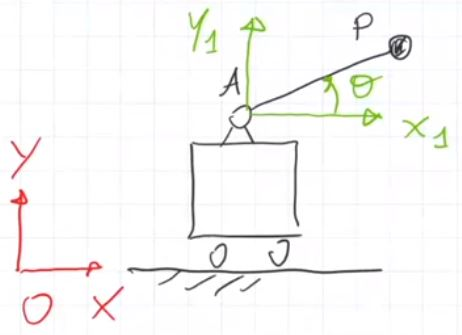
\includegraphics[height=3cm]{../lezione3/img1.JPG}
\end{center} 
L'immagine mostra un carrello su cui è incernierata una barra $AP$. Se andiamo a considerare un unico sistema di riferimento assoluto (in rosso), il moto del punto $P$ è un moto rototraslatorio, ma, se noi andassimo a inserire un sistema di riverimento mobile (in verde) che trasla insieme al punto $A$, il moto del punto $P$ diventa un moto di rotazione. Abbiamo dunque scomposto il moto rototraslatorio del punto $P$ nel moto traslatorio del nuovo sistema di riferimento mobile e nel moto rotatorio del punto $P$ in questo nuovo sistema di riferimento.\newline
\rule{\textwidth}{0,4pt}
\newline
\textbf{es.}\newline
[immagine dagli appunti del prof]
\begin{center}
    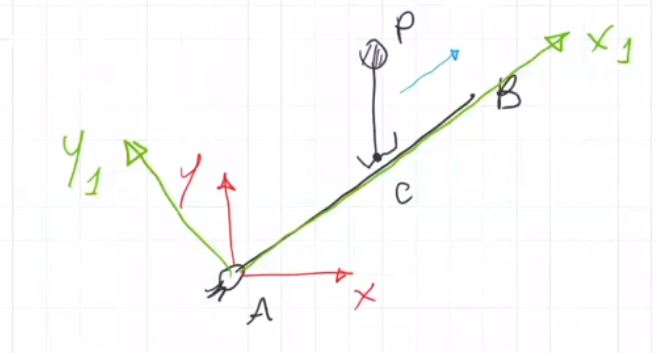
\includegraphics[height=3cm]{../lezione3/img2.JPG}
\end{center}
L'immagine mostra un asta $AB$ incernierata al pavimento che può ruotare, sull'asta può, inoltre, scivolare una seconda asta $CP$. Anche in questo caso il moto del punto $P$ rispetto a un unico sistema di riferimento assoluto (in rosso) sarebbe un moto rototraslatorio. Se però introduciamo un sistema di riferimento mobile (in verde) che abbia assi $Y_1$ e $X_1$ che ruotano insieme all'asse $AB$, il moto del punto $P$ diventa un moto traslatorio.\newline
\rule{\textwidth}{0,4pt}
\subsection{Posizione}
[immagine dagli appunti del prof]
\begin{center}
    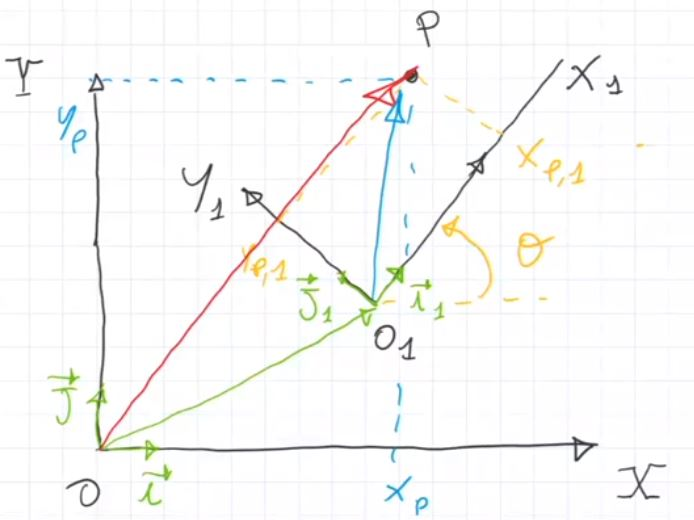
\includegraphics[height=5cm]{../lezione3/img3.JPG}
\end{center}
Vogliamo descrivere il moto di un generico punto $P$ (velocità, posizione, accellerazione) andando a introdurre un nuovo sistema di riferimento mobile ($O_1, X_1, Y_1$) rispetto a un sistema di riferimento fisso ($O, X, Y$).\newline
Il sistema di riferimento mobile introdotto è in moto rototraslatorio noto rispetto al sistema di riferimento assoluto.\newline
Indichiamo con $\theta$ la rotazione del sistema di riferimento mobile rispetto al sistema di riferimento assoluto.\newline
\newline 
Il punto generico $P$ ha coordinate $x_P, y_P$ rispetto al sistema assoluto, e $x_{P,1}, y_{P,1}$ rispetto al sistema mobile. \newline
\newline
La posizione può essere vista come somma vettoriale (come abbiamo visto per i corpi rigidi): 
\[
    (P-O) = (O_1 - O) + (P-O_1)
\]
dove $(P-O) = x_P \vec{i} + y_P \vec{j}$ e $(O_1 - O) = x_{O_1} \vec{i} + y_{O_1} \vec{j}$ e $(P-O_1) = x_{P,1} \vec{i_1} + y_{P,1} \vec{j_1}$. Se il moto del sistema di riferimento mobile è noto, conoscendo la posizione di $P$ rispetto al sistema assoluto, posso ricavare la posizione rispetto al sistema mobile, viceversa, conoscendo la posizione di $P$ rispetto al sistema mobile, posso ricavare la posizione rispetto al sistema assoluto.
\[
    (P-O) = x_{O_1}\vec{i} + y_{O_1}\vec{j} + x_{P,1} \vec{i_1} + y_{P,1} \vec{j_1}
\]
\subsection{Velocità}
La velocità è definita come $\vec{v_P} = \frac{d}{dt} (P-O) = \frac{d}{dt} (O_1 - O) + \frac{d}{dt} (P-O_1)$, sviluppando queste derivate, otteniamo: 
\[
    \vec{v_P} = 
        \dot{x}_{O_1}\vec{i} + 
        \dot{y}_{O_1} \vec{j} + 
        \dot{x}_{P,1} \vec{i_1} + 
        \dot{y}_{P,1} \vec{j_1} + 
        x_{P,1} \frac{d}{dt}\vec{i_1} + 
        y_{P,1} \frac{d}{dt} \vec{j_1}
\]
\ \newline
In teoria, i primi due termini, se $\vec{i}$ e $\vec{j}$ variassero il loro orientamento rispetto al tempo, dovrebbero essere derivati pure loro, ma siccome il sistema di riferimento assoluto è fisso, la loro derivata è nulla.\newline
Per i secondi due termini invece i versori variano il proprio orientamento nel tempo perchè fanno riferimento a un sistema mobile, dunque non posso trascurare la loro derivata e per questo ci sono gli ultimi due addendi.\newline
\newline
1- La prima coppia di termini $\dot{y}_{O_1} \vec{j} + \dot{x}_{P,1} \vec{i_1}$ rappresenta la velocità $\vec{v}_{O_1}$ del punto $O_1$ rispetto al sistema di riferimento assoluto, anche detta velocità assoluta di $O_1$.\newline
2- La seconda coppia di termini $\dot{y}_{P,1} \vec{j_1} + x_{P,1} \frac{d}{dt}\vec{i_1}$ rappresenta la velocità $\vec{v}_{rel, P}$ relativa di $P$, cioè la velocità di $P$ rispetto al sistema di riferimento mobile.\newline
3- La terza e ultima coppia $x_{P,1} \frac{d}{dt}\vec{i_1} + y_{P,1} \frac{d}{dt} \vec{j_1}$ è più complicata da analizzare e dobbiamo prima capire cosa sono le derivate dei versori $\vec{i_1}$ e $\vec{j_1}$.\newline
\newline
[immagine dagli appunti del prof]
\begin{center}
    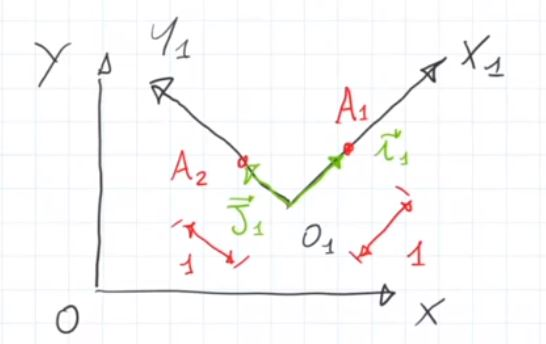
\includegraphics[height=3cm]{../lezione3/img4.JPG}
\end{center}
Consideriamo i due sistemi di riferimento, mobile e assoluto, e poniamo due punti $A_1$ e $A_2$ sugli assi del sistema di riferimento mobile a distanza unitaria dall'origine $O_1$. Questi due punti rappresentano i nostri versori $\vec{j_1}$ e $\vec{i_1}$.
\[
    (A_1 - O) = (O_1-O) + (A_1 - O_1) \;\text{, dove il termine $(A_1-O_1)$ è il versore $\vec{i_1}$}\;
\]
\[
    (A_2 - O) = (O_1-O) + (A_2 - O_1) \;\text{, dove il termine $(A_2-O_1)$ è il versore $\vec{j_1}$}\;
\]
Andiamo a derivare queste due equazioni per determinare la velocità dei punti $A_1$ e $A_2$. Facciamo i calcoli solo per $A_1$, per $A_2$ i procedimenti sono del tutto analoghi:
\[
    \frac{d}{dt}(A_1-O) = \frac{d}{dt}(O_1 - O) + \frac{d}{dt}(A_1 -O_1)
\]
Il termine $\frac{d}{dt}(A_1-O)$ rappresenta la velocità assoluta $\vec{v}_{A_1}$ di $A_1$, il secondo termine $\frac{d}{dt}(O_1 - O)$ è la velocità assoluta $\vec{v}_{O_1}$ di $O_1$, l'ultimo termine $\frac{d}{dt}(A_1 -O_1)$ è la derivata $\frac{d}{dt}\vec{i_1}$ rispetto al tempo del versore $\vec{i_1}$. Abbiamo quindi determinato la velocità assoluta del punto $A_1$.\newline
\newline
Potevamo ottenere il medesimo risultato usando il terorema di Rivals per un corpo rigido (che in questo caso è rappresentato dal sistema di riferimento mobile), infatti la velocità di un punto qualsiasi di un corpo rigido è data dalla somma di due componenti: una componente di traslazione di un punto generico del corpo (per esempio l'orgine $O_1$) e una componente di rotazione del corpo attorno al punto $O_1$. Se andiamo a definire il vettore velocità angolare $\vec{\omega} = \dot{\theta} \vec{k} = \omega \vec{k} = \omega \vec{k_1}$ del sistema mobile, allora
\[
    \vec{v}_{A_1} = \vec{v}_{O_1} + \vec{\omega} \land (A_1 - O_1) =\;\text{[dove $(A_1 - O_1) = \vec{i_1}$]}\; = \vec{v}_{O_1} + \vec{\omega}\land \vec{i_1}
\]
\newline
Riprendendo entrambi i metodi visti e uguagliandoli, otteniamo:
\[
    \vec{v}_{A_1} = \cancel{\vec{v}_{O_1}} + \frac{d}{dt}\vec{i_1} = \cancel{\vec{v}_{O_1}} + \vec{\omega} \land \vec{i_1} \Longrightarrow \frac{d}{dt}\vec{i_1} = \vec{\omega}\land \vec{i_1}
\]
\ \newline
Procedendo in maniera analoga anche per il punto $A_2$, otteniamo le \textbf{formule di Poisson}
\[
    \begin{cases}
        \frac{d}{dt}\vec{i_1} = \vec{\omega}\land \vec{i_1}\\
        \\
        \frac{d}{dt}\vec{j_1} = \vec{\omega}\land \vec{j_1}
    \end{cases}
\]
Possiammo ora andare a sostituirle all'interno della formula della velocità scritta in precedenza ($
    \vec{v_P} = 
        \dot{x}_{O_1}\vec{i} + 
        \dot{y}_{O_1} \vec{j} + 
        \dot{x}_{P,1} \vec{i_1} + 
        \dot{y}_{P,1} \vec{j_1} + 
        x_{P,1} \frac{d}{dt}\vec{i_1} + 
        y_{P,1} \frac{d}{dt} \vec{j_1}
$):
\[
    \vec{v_P} = 
        \vec{v}_{O_1} + \vec{v}_{rel, P} +
        x_{P,1} \vec{\omega}\land \vec{i_1} + 
        y_{P,1} \vec{\omega}\land \vec{j_1}
\]
dove i termini $x_{P,1} \vec{\omega}\land \vec{i_1} + y_{P,1} \vec{\omega}\land \vec{j_1}$ possono essere riscritti come $\vec{\omega}(x_{P,1} \vec{i_1} + y_{P,1} \vec{j_1})$ (la parentesi rappresenta il vettore $(P-O_1)$.\newline
\newline
\textbf{teor.} \textbf{Teorema dei moti relativi per le velocità}
\[
    \vec{v_P} = 
        \vec{v}_{O_1} + \vec{v}_{rel, P} + \vec{\omega} \land (P-O_1) = 
        \vec{v}_{tr,P} + \vec{v}_{rel, P}
\]
dove la somma di $\vec{v}_{O_1} + \vec{\omega} \land (P-O_1)$ prende il nome di \textbf{velocità di trascinamento} $\vec{v}_{tr,P}$ del punto $P$, che è la velocità che il punto $P$ avrebbe se fosse rigidamente collegato al sistema di riferimento mobile.\newline
Questo teorema esprime la relazione fra la velocità assoluta di un punto $P$ e la \textbf{velocità relativa} a un sistema di riferimento in moto relativo rispetto a quello assoluto. La velocità assoluta è quindi la somma di due componenti, la velocità di trascinamento e la velocità relativa rispetto al sistema mobile.\newline
Quindi una volta noto il moto di trascinamento del sistema mobile è possibile passare dalla velocità assoluta a quella relativa e viceversa.
\subsection{Accellerazione}
Anche per l'accellerazione vogliamo cercare una relazione fra l'accellerazione del punto $P$ rispetto al sistema di riferimento assoluto e l'accellerazione del punto $P$ rispetto al sistema di riferimento mobile.\newline
\newline
Deriviamo dunque rispetto al tempo l'equazione $\vec{v_P} = \vec{v}_{O_1} + \vec{v}_{rel, P} + \vec{\omega} \land (P-O_1)$:
\[
    \vec{a}_P = \frac{d}{dt} \vec{v}_P = \frac{d}{dt} \vec{v}_{O_1} + \frac{d}{dt}(\vec{\omega}\land (P-O_1)) + \frac{d}{dt}\vec{v}_{rel,P}
\]
Deriviamo questi ultimi tre addendi singolarmente:
\begin{itemize}
    \item Il primo termine $\frac{d}{dt} \vec{v}_{O_1}$ è l'accellerazione $\vec{a}_{O_1}$ assoluta del punto $O_1$.
    \item Il secondo termine, cioè la derivata rispetto al tempo $\frac{d}{dt}(\vec{\omega}\land (P-O_1))$, si ottiene derivando prima il vettore omega rispetto al tempo e moltiplicandola per il vettore $P-O_1$ e successivamente moltiplicando omega per la derivata rispetto al tempo del vettore $(P-O_1)$. Quindi otteniamo $\frac{d}{dt}(\vec{\omega}\land (P-O_1)) = \dot{\vec{\omega}} \land (P-O_1) + \vec{\omega} \frac{d}{dt}(P-O_1)$, dove $\dot{\vec{\omega}} = \ddot{\theta} \vec{k}$. Possiamo quindi riscrivere questo secondo termine come $\dot{\vec{\omega}} \land (P-O_1) + \vec{\omega}\land \vec{v}_{rel,P} + \vec{\omega} + \vec{\omega}\land[\vec{\omega \land (P-O_1)}]$.
    \item Sapendo che $\vec{v}_{rel,P} = \dot{x}_{P,1} \vec{i_1} + \dot{y}_{P,1} \vec{j_1}$, possiamo derivare il terzo termine, derivando sia $\dot{x}_{P,1}$ e $\dot{y}_{P,1}$, sia i versori $\vec{i_1}$ e $\vec{j_1}$ perchè sono versori di un sistema di riferimento in movimento.\newline
    Quindi otteniamo $\frac{d}{dt}\vec{v}_{rel,P} = \ddot{x}_{P,1} \vec{i_1} + \ddot{y}_{P,1} \vec{j_1} + \dot{x}_{P,1} \frac{d}{dt} \vec{i_1} + \dot{y}_{P,1} \frac{d}{dt}\vec{j_1}$, dove i primi due addendi sono l'accellerazione $\vec{a}_{rel,P}$ relativa del punto $P$ e gli ultimi due addendi possono essere riscritti grazie alle formule di Poisson nel seguente modo: $\dot{x}_{P,1} \frac{d}{dt} \vec{i_1} + \dot{y}_{P,1} \frac{d}{dt}\vec{j_1} = \dot{x}_{P,1} \vec{\omega}\land \vec{i_1} + \dot{y}_{P,1} \vec{\omega}\land \vec{j_1} = \vec{\omega} \land (\dot{x}_{P,1} \vec{i_1} + \dot{y}_{P,1} \vec{j_1})$, inoltre il termine fra parentesi è la velocità $\vec{v}_{rel,P}$ relativa del punto $P$.
\end{itemize}
\textbf{teor.} \textbf{Teorema dei moti relativi per le accellerazioni o teorema di Coriolis}:
\[
    \vec{a}_P = \vec{a}_{O_1} + \dot{\vec{\omega}} \land (P-O_1) + \vec{\omega} \land [\vec{\omega}\land (P-O_1)] + 2 \cdot \vec{\omega}\land \vec{v}_{rel,P} + \vec{a}_{rel,P}
\]
Nei primi tre termini ($\vec{a}_{O_1} + \dot{\vec{\omega}} \land (P-O_1) + \vec{\omega} \land [\vec{\omega}\land (P-O_1)]$) si riconosce il teorema di Rivals per le accellerazioni relative a un punto $P$ che si muove solidalmente con la terna mobile. $\vec{a}_{O_1}$ è l'accellerazione con cui la terna si sposta; $\vec{a}_{tg,P} = \dot{\vec{\omega}} \land (P-O_1)$ e $\vec{a}_{n,P} = \vec{\omega} \land [\vec{\omega}\land (P-O_1)]$ sono l'accellerazione legata al moto rotatorio di $P$ attorno ad $O_1$, in particolare il primo è la componente tangenziale, e il secondo la componente normale. I tre termini assieme sono \textbf{l'accellerazione di trascinamento} $\vec{a}_{tr,P}$ del punto $P$, cioè l'accellerazione che avrebbe il punto $P$ se fosse rigidamente legato al sistema di riferimento mobile.\newline
A questo termine di accellerazione di trascinamento vengono aggiunte un'\textbf{accellerazione relativa} $\vec{a}_{rel,P}$ (come accade anche per la velocità) e il termine $\vec{a}_{co} = 2 \cdot \vec{\omega}\land \vec{v}_{rel,P}$ detto \textbf{accellerazione complementare o di Coriolis} (di cui non c'è il rispettivo per la velocità).
\[
    \vec{a}_P = \vec{a}_{tr,P} + \vec{a}_{co} + \vec{a}_{rel,P}
\]
\[
    \begin{cases}
        \vec{a}_{tr,P} = \vec{a}_{O_1} + \dot{\vec{\omega}} \land (P-O_1) + \vec{\omega} \land [\vec{\omega}\land (P-O_1)]\\
        \vec{a}_{co} = 2 \cdot \vec{\omega}\land \vec{v}_{rel,P}\\
        \vec{a}_{rel,P} = \vec{a}_{rel,P}
    \end{cases}
\]
Notiamo che l'accellerazione di Coriolis $\vec{a}_{co}$ si annulla per tre casi: 
\begin{itemize}
    \item $\vec{\omega} \parallel \vec{v}_{rel,P}$ (impossibile nel piano);
    \item $\vec{\omega} = 0$ (il sistema mobile si muove di moto traslatorio);
    \item $\vec{v}_{rel,P} = 0$, in questo caso il teorema di Coriolis coincide con il teorema di Rivals.
\end{itemize}
\newpage
\section{Sistemi meccanici}
In prima approssimazione possiamo vedere una macchina come un insieme di corpi rigidi legati fra loro attraverso opportuni vincoli. I vincoli sono condizioni essenziali per lo studio di una macchina e devono sempre essere rispettati.\newline
Esistono vincoli \textbf{interni}, cioè legati ai corpi rigidi del sistema, o \textbf{esterni}, cioè legati alla struttura che contiene questi corpi rigidi, chiamata \textbf{telaio}.
\subsection{Vincoli elementari}
In questo corso andremo ad analizzare solo i vincoli elementari, che sono dei vincoli che realizzano la diretta soppresione di uno o più gradi di libertà di un corpo, cioè vanno ad inibire una delle possibilità di moto del corpo rigido. Ricordiamo che il corpo rigido nel piano ha tre gradi di libertà, le traslazioni degli assi $X$ e $Y$ e la rotazione.\newline
Un vincolo che impedisce $n$ gradi di libertà, viene espresso algebricamente come $n$ equazioni vincolanti.
\subsubsection{Vincoli tripli}
E' un vincolo che sopprime tutte le possibilità di moto di un corpo rigido.
\begin{itemize}
    \item \textbf{Incastro}: [immagine dagli appunti del prof]
    \begin{center}
        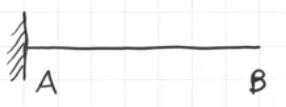
\includegraphics[height=1.5cm]{../lezione3/img5.JPG}
    \end{center}
    Vediamo una trave $AB$ incastrata nel punto $A$ che non ha più possibilità di movimento. 
\end{itemize}
\subsubsection{Vincoli doppi}
Sono vincoli che sopprimo due possibilità di moto di un corpo rigido, che avrà quindi ancora una possibilità di moto disponibile.
\begin{itemize}
    \item \textbf{Cerniera}: [immagine dagli appunti del prof]
    \begin{center}
        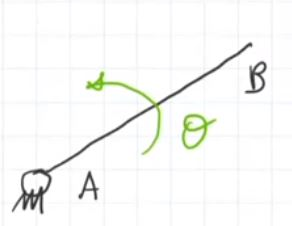
\includegraphics[height=3cm]{../lezione3/img6.JPG}
    \end{center}
    Vediamo una trave $AB$ con una cerniera nel punto $A$. La cerniera impedisce ogni traslazione possibile, tuttavia la trave può ancora ruotare.
    \item \textbf{Pattino}: [immagine dagli appunti del prof]
    \begin{center}
        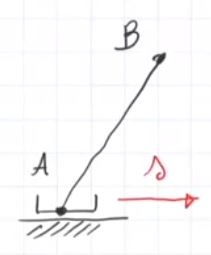
\includegraphics[height=3cm]{../lezione3/img7.JPG}
    \end{center}
    Vediamo una trave $AB$ con un pattino nel punto $A$. Il pattino impedisce il distacco dalla linea piana e impedisce anche ogni rotazione, tuttavia la trave può ancora scivolare sulla guida che si sta considerando.
    \item \textbf{Manicotto}: [immagine dagli appunti del prof]
    \begin{center}
        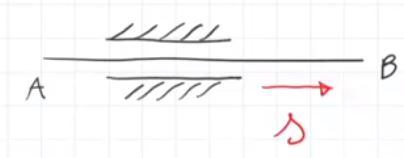
\includegraphics[height=2cm]{../lezione3/img8.JPG}
    \end{center}
    Vediamo una trave $AB$ a cui è imposto un vincolo manicotto. Il manicotto impedisce rotazioni e movimenti perpendicolari, tuttavia la trave può ancora scivolare in direzione parallela.
\end{itemize}
\subsubsection{Vincoli singoli}
Sono vincoli che sopprimo una sola possibilità di moto di un corpo rigido.
\begin{itemize}
    \item \textbf{Carrello più cerniera o carrello}: [immagine dagli appunti del prof]
    \begin{center}
        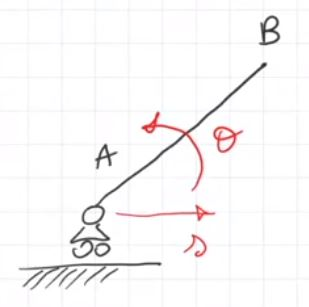
\includegraphics[height=3cm]{../lezione3/img9.JPG}
    \end{center}
    Vediamo una trave $AB$ con un carrello più cerniera nel punto $A$. Il carrello più cerniera impedisce unicamente movimenti perpendicolari alla guida, ma consente spostamenti paralleli alla guida o rotazioni.
\end{itemize}